\chapter{Quick start}\label{QuickStart}

Starting \GS\ for the first time you get an opening screen. And then?
This will give you a quick introduction to get started with some suggestions on how to use it but without explaining too much. All the explaining is done in subsequent chapters.
For full details on all screen details, buttons and text see chapter \nameref{ScreensMenuButtons}. buttons'%\Chapref{Screens, menu and buttons}'.

\begin{figure}[h!]
    \centering
    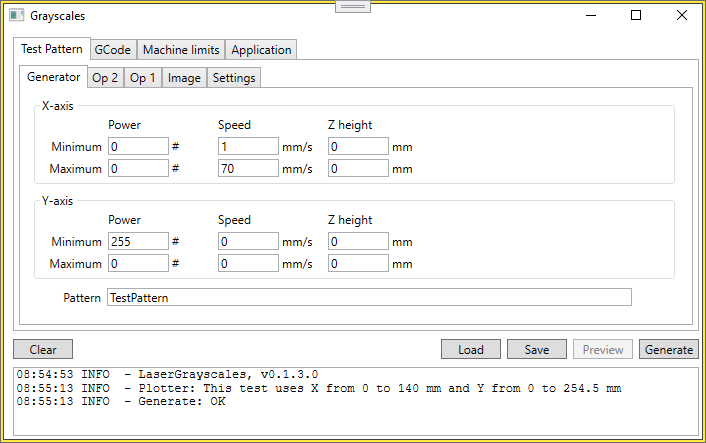
\includegraphics[width=0.8\linewidth]{./images/Grayscales-v0.1.3.png}
\end{figure}

\section{Configuration}
Starting for the first time a configuration for `Stepcraft, D3/600' using `UCCNC' is assumed.

If you are not using a `Stepcraft, D3/600' machine see the tab `Machine limits' and check that the limit settings comply with your machine. Change settings accordingly. This needs to be done only once.

If you are not using `UCCNC' as GCode interpreter see the tab `GCode' and check that configured GCode comply with your interpreter. Change settings accordingly. This needs to be done only once.

You can skip these first two steps and still generate test patterns but the GCode for it might well be violating your machine limits or be invalid for your interpreter. This also might be the case
if you do make the first to steps but made some errors or oversights.

\WarningCheckAndTest

\section{Test script}
The default test script is set for an image of 0 to 140 mm on the X-axis and 0 to 255 mm on the Y-axis, Z is fixed at 0 mm.

The image is 255 continues lines in the X direction, separated by 0.5 mm in the Y direction.
In the X direction speed (for G1) is changed from 1 to 70 mm/sec (60 to 4200 mm/min) and in the Y direction laser power is changed from 255 (100\%) to 0 (0\%).

In the tab `Image' you see details for the line segments, by default a line segment (written at a fixed speed an laser power) is 2 mm long (in the X direction) and the next line (in the Y direction)
is 0.5 mm above it. These two settings have a major influence on the final width and height of the image and also on that what you want to test. In stead of lines you can also use squares, blocks or images.

In the tab `Op 1' (for Operation 1) you see that in the X direction there is no gap between the images and that it is repeated 70 times. In the Y direction there is an additional gap 0f 0.5 mm.
Tab `Op 2' is similar and defines one image (no repeats) and defining a gap here does not do anything.

To arrange grouping of 8 lines one can define an Image count of 8 in the y direction on the `Op 1' tab and an Image count of 32 in the y direction with an appropriate gap on the `Op 2' tab.

At the `Generator' tab the settings for Power, Speed and Z-height for each image is defined. This is done for both the X direction and the Y direction. The actual value used is the sum of both.
By default the Z-height is at a constant value of 0.

The speed is changed van 1 to 70 mm/s (60 to 420 mm/min) in the X direction. There are 70 line segment images in the X direction thus each
image in the X direction is done 1 mm/sec (60 mm/min) faster than the previous one.

The laser power is changed from 0 to 255 in the Y direction. There are 255 lines in the Y direction thus each image in the Y direction is using one step of laser power more than the previous one.

The text field `Pattern' is used for the name of the generated pattern. This name is appended with a date/time stamp.

\section{Generating a script}
After checking all settings it is time to generate the test script. Press the button `Generate' and a script is written to `.\textbackslash{}build\textbackslash{}TestPattern-yyyy-MM-ddTHH.mm.ss.nc'

With the `Save' button you can save all your test settings in a file, with `Load' you can load it again. The button `Preview' is for future use.

At the bottom of the form you can follow the progress of generating the script and look at some details for invalid values. Generating the standard script with lines will take a few seconds
depending on PC capabilities. It is reasonable to expect something at or below 10 seconds, a time of one minute is unrealistic long.
%When using the same settings for a standard script and apply it to a square it will take a prohibitive amount of time (and memory). Try a small pattern first and see how fast how many lines
%it generates. Progressively make it bigger until you get what you need or when time, memory or lines become unacceptable large.

\section{Reducing script processing time}
Executing the GCode from the default script takes a lot more time and a lot of material, both considerd to be scarce resources. On a Stepcraft D3/600 a processing time of around one hour is
to be expected. A surface of 140 x 255 mm of some (possible expensive) material does not feel right either. With common sense there are several options to reduce this time. The script is
configured to take one unit step for speed and laser poser and run over the full scale of it.

First suggestion is not to run over the full scale but only over the part that is about right, say a speed of 30 to 60 mm/sec  (1800 to 3600 mm/min) and a laser power range of 100 to 200
(about 40\% to 80\% of full laser power). That on its own is not sufficient. Also reduce the number of copies in `Op 1' (and in `Op 2' if you are using it) to a total of say 10 in each direction
This will give a big reduction is processing time bringing it back to the range of minutes. But it also produce a more coarse result. With this result you may be able to select the rough settings
of speed an laser power for an optimal result and generate a second test around these values.

This way it is possible to get good estimates of settings using a minimum abound of time and material.
